\documentclass[reprint,english,notitlepage,aps,nobalancelastpage,nofootinbib]{revtex4-1}
\usepackage[utf8]{inputenc}
\usepackage[english]{babel}
\usepackage{physics,amssymb}
\usepackage{graphicx}
\usepackage{xcolor}
\usepackage{hyperref}
\usepackage{tikz}
\usepackage{listings}
\usepackage{subfigure}
\usepackage{amsmath,mathtools}
\usepackage{amsbsy}
\usepackage{enumitem}
\usepackage{bbold}

\graphicspath{{../plots/}}

\hypersetup{
    colorlinks,
    linkcolor={red!50!black},
    citecolor={blue!50!black},
    urlcolor={blue!80!black}}

\lstset{
	inputpath=,
	backgroundcolor=\color{white!88!black},
	basicstyle={\ttfamily\scriptsize},
	commentstyle=\color{magenta},
	language=Python,
	morekeywords={True,False},
	tabsize=4,
	stringstyle=\color{green!55!black},
	frame=single,
	keywordstyle=\color{blue},
	showstringspaces=false,
	columns=fullflexible,
	keepspaces=true}


\newcommand{\closed}[1]{\left(#1\right)}
\newcommand{\bracket}[1]{\left[#1\right]}

\newcommand{\kt}{\kappa_T}
\renewcommand{\cp}{c_P}
\newcommand{\cv}{c_V}
\renewcommand{\a}{\alpha}

\newcommand{\tmdv}[4]{\closed{\pdv{#1}{#2}}_{#3,#4}}
\newcommand{\jacobian}[2]{\pdv{(#1)}{(#2)}}
\renewcommand{\d}{\mathrm{d}}

\newcommand{\nx}{N_x}
\newcommand{\ny}{N_y}
\newcommand{\nz}{N_z}
\newcommand{\V}{\tilde{V}}
\renewcommand{\P}{\tilde{P}}

\newcommand{\np}{N_+}
\newcommand{\kb}{k_B}

\begin{document}
\begin{center}
\title{\Huge FYS4130 - Oblig 1}
\author{\large Vetle A. Vikenes}
\date{\today}
\noaffiliation


\maketitle
\end{center}
\onecolumngrid

\section*{\large Task 1 - Black box numerical method}
We want to find the isothermal compressibility at constant $T$ and $N$,
\begin{align} \label{eq:kappa black box}
	\kt = -\frac{1}{V}\closed{\pdv{V}{P}}_{T,N},
\end{align}
with a black box numerical method which gives us values for $P$ and $N$ as function of intput parameters $T,\,V,$ and $\mu$ which we may vary. The derivatives we're able to compute with our numerical method is the partial derivative of either $P$ or $N$ with respect to one of the input parameters, when the other two are held constant. We must therefore rewrite equation \eqref{eq:kappa black box}, such that it only contains such derivatives. To begin, we use the chain rule on the reciprocal of the partial derivative in equation \eqref{eq:kappa black box}
\begin{align*}
	\tmdv{P}{V}{T}{N} &= \jacobian{P,T,N}{V,T,N}=\jacobian{P,T,N}{V,T,\mu}\cdot\jacobian{V,T,\mu}{V,T,N} \\
	&= \jacobian{P,N,T}{V,\mu,T}\cdot\jacobian{\mu,V,T}{N,V,T}=
	\jacobian{P,N,T}{V,\mu,T} \Big/ \tmdv{N}{\mu}{V}{T}.
\end{align*}
The last factor is a partial derivative we're able to compute, by computing the change in $N$ as we vary $\mu$ only. For the other factor, we expand the jacobian, using its definition 

\begin{align}
	\jacobian{P,N,T}{V,\mu,T} &= \tmdv{P}{V}{\mu}{T}\tmdv{N}{\mu}{V}{T}-\tmdv{P}{\mu}{V}{T}\tmdv{N}{V}{\mu}{T}. \label{eq:d PNT_d VmuT}
\end{align}
We see that the four partial derivatives in equation \eqref{eq:d PNT_d VmuT} are taken with respect to either $V$, with the other input parameters held constant, or $\mu$ with the other input parameters held constant. Measuring the change in $P$ and $N$ with these constraints is thus something our numerical method is capable of, and we have successfully reduced $\kt$ into multiple partial derivatives we're able to solve. The resulting expression for $\kt$ becomes  

\begin{align*}
	\kt &= -\frac{1}{V}\bracket{\jacobian{P,N,T}{V,\mu,T} \Big/ \tmdv{N}{\mu}{V}{T}}^{-1}=-\frac{1}{V} \tmdv{N}{\mu}{V}{T} \Big/
	\jacobian{P,N,T}{V,\mu,T} \\
	&= -\frac{1}{V} \tmdv{N}{\mu}{V}{T} \bracket{\tmdv{P}{V}{\mu}{T}\tmdv{N}{\mu}{V}{T}-\tmdv{P}{\mu}{V}{T}\tmdv{N}{V}{\mu}{T}}^{-1}.
\end{align*}

\section*{\large Task 2 - Partial derivative}
We want to rewrite the partial derivative 
\begin{align*}
	\tmdv{P}{U}{G}{N}.
\end{align*}
In this task we will need the standard set of second derivatives given in Swendsen, and we list them here for convenience
\begin{align}
	\a &= \frac{1}{V} \tmdv{V}{T}{P}{N} \label{eq:alpha} \\ 
	\kt &= -\frac{1}{V} \tmdv{V}{P}{T}{N} \label{eq:kappa} \\ 
	\cp &= \frac{T}{N} \tmdv{S}{T}{P}{N} \label{eq:cp} \\ 
\end{align}
We begin by applying the chain rule to the Jacobian, which enables us to get a partial derivative containing $U$ and $G$ in the denominator only. 

\begin{align} 
	\tmdv{P}{U}{G}{N} &= \jacobian{P,G,N}{U,G,N} = \jacobian{P,G,N}{P,T,N}\cdot\jacobian{P,T,N}{U,G,N}= \tmdv{G}{T}{P}{N} \jacobian{P,T,N}{U,G,N} \nonumber \\
	&= -S \Big/\jacobian{U,G,N}{P,T,N}, \label{eq:pdv first expansion}
\end{align}
where we used the differential form of the Gibbs free energy, $\mathrm{d}G=-S\mathrm{d}T+V\mathrm{d}P+\mu\mathrm{d}N$, to solve the first partial derivative of $G$ with respect to $T$ at constant $P$ and $N$. The second factor was written in terms of the reciprocal such that the thermodynamic potentials in the Jacobian appear in the nominator. 

We will now find an expression for $\pdv*{(U,G,N)}{(P,T,N)}$. To avoid partial derivatives containing $U$ and $G$ simultaneously, we expand the expression by using the definition of Jacobians. 

\begin{align}
	\jacobian{U,G,N}{P,T,N} &= \tmdv{U}{P}{T}{N} \tmdv{G}{T}{P}{N} - \tmdv{U}{T}{P}{N}\tmdv{G}{P}{T}{N} \nonumber \\ 
	&= -S\tmdv{U}{P}{T}{N} - V \tmdv{U}{T}{P}{N}, \label{eq:d UGN_d PTN}
\end{align}
where the last equation follow from the definition of $\d G$ and the partial derivatives of it. 

For the partial derivative of $U$ with respect to $T$ at constant $P$ and $N$, we consider the differential form of fundamental relation in the energy representation, which at constant $N$ becomes 

\begin{align}
	\d U &= T \d S - P \d V \nonumber \\ 
	\implies \tmdv{U}{T}{P}{N} &= T \tmdv{S}{T}{P}{N} - P \tmdv{V}{T}{P}{N} \nonumber \\ 
	&= N\cp - PV\a, \label{eq:dU_dT}
\end{align}
where we used equations \eqref{eq:cp} and \eqref{eq:alpha} for the two partial derivatives. 

For the partial derivative of $U$ with respect to $P$ with $T$ and $N$ held constant we apply the chain rule
\begin{align}
	\tmdv{U}{P}{T}{N} &= \jacobian{U,T,N}{P,T,N} = \jacobian{U,T,N}{V,T,N}\cdot \jacobian{V,T,N}{P,T,N} = \tmdv{U}{V}{T}{N} \tmdv{V}{P}{T}{N} \nonumber \\
	&= \tmdv{U}{V}{T}{N}(-V\kt). \label{eq:dU_dP}
\end{align}
Equation \eqref{eq:kappa} was used to rewrite the second partial derivative. For the other partial derivative, we once again use the previouslly mentioned expression for $\d U$ with $N$ held constant 
\begin{align} \label{eq:dU_dV}
	\tmdv{U}{V}{T}{N} &= T \tmdv{S}{V}{T}{N} - P.
\end{align}
To proceed with the final partial derivative we will first use a Maxwell relation. We notice that $S$ is differentiated with respect to $V$ at constant $T$ and $N$, so we can use the differential form of the Helmholtz free energy to derive the Maxwell relation. 
\begin{align*}
	\d F &= -S \d T -P \d V + \mu \d N \implies -\tmdv{F}{T}{V}{N} = S \\ 
	\tmdv{S}{V}{T}{N} &=-\bracket{\pdv{V}\tmdv{F}{T}{V}{N}}_{T,N} = -\bracket{\pdv{T}\tmdv{F}{V}{T}{N}}_{V,N} = \tmdv{P}{T}{V}{N}.
\end{align*} 
We rewrite the last partial derivative using the chain rule 
\begin{align}
	\tmdv{P}{T}{V}{N} &= \jacobian{P,V,N}{T,V,N} = \jacobian{P,V,N}{P,T,N}\cdot \jacobian{P,T,N}{T,V,N} = -\jacobian{V,P,N}{T,P,N}\cdot \jacobian{P,T,N}{V,T,N} \nonumber \\ 
	&= -\tmdv{V}{T}{P}{N} \Big/ \tmdv{V}{P}{T}{N} = -V\a \big/ (-V\kt) = \frac{\a}{\kt}, \label{eq:alpha_kappa}
\end{align} 
where in the last step equations \eqref{eq:alpha} and \eqref{eq:kappa} were used to rewrite the nominator and denominator, repsectively. Equation \eqref{eq:dU_dP} can now be solved, by inserting equation \eqref{eq:alpha_kappa} into equation \eqref{eq:dU_dV} 
\begin{align*}
	\tmdv{U}{P}{T}{N} &= -V\kt \tmdv{U}{V}{T}{N} = -V\kt \closed{T\frac{\a}{\kt} - P} \\ 
	&= -VT \a + PV\kt 
\end{align*}

Inserting equation \eqref{eq:dU_dP} and \eqref{eq:dU_dT} into equation \eqref{eq:d UGN_d PTN} we get 
\begin{align}
	\jacobian{U,G,N}{P,T,N} = -S \closed{-VT \a + PV\kt} - V \closed{N\cp - PV\a} = -V\bracket{SP\kt + N\cp -ST\a - PV\a} \label{eq:d UGN_d PTN final expression}
\end{align}

Finally, inserting equation \eqref{eq:d UGN_d PTN final expression} into equation \eqref{eq:pdv first expansion} we arrive at the final expression 
\begin{align}
	\tmdv{P}{U}{G}{N} &= -S \bracket{\jacobian{U,G,N}{P,T,N}}^{-1} = \frac{S/V}{SP\kt + N\cp -ST\a - PV\a}
\end{align}


\section*{\large Task 3}
We consider the Helmholtz free energy given by equation \eqref{eq:F_task3}
\begin{align} \label{eq:F_task3}
	F = T \bracket{N_x \ln\closed{\a l b^2 \frac{N_x}{{V}}} + N_y \ln\closed{\a l b^2 \frac{N_y}{{V}}} + N_z \ln\closed{\a l b^2 \frac{N_z}{{V}}} + \gamma l b^2 \frac{\nx\ny+\ny\nz+\nz\nx}{{V}} }
\end{align}

\subsection*{a) - Dimensionless volume}
Using $\tilde{V}=V/lb^2$, we can rewrite the four volume terms in the expression by $lb^2/V=1/\tilde{V}$. The expression for the Helmholtz free energy divided by $T$ now becomes 
\begin{align*} 
	\frac{F}{T} = \bracket{N_x \ln\closed{\a  \frac{N_x}{\tilde{V}}} + N_y \ln\closed{\a  \frac{N_y}{\tilde{V}}} + N_z \ln\closed{\a  \frac{N_z}{\tilde{V}}} + \gamma \frac{\nx\ny+\ny\nz+\nz\nx}{\tilde{V}} }
\end{align*}

\subsection*{b) - Equilibrium Helmholtz free energy}
We will now increase the rod concentration, $n=N/V$, so slow that we always consider the system to be in equilibrium. The temperature and volume is kept constant, but we increase $N$ by adding rods. We will set $\alpha=1$ in all following calculations.  
\begin{align} \label{eq:F_dimless}
	\frac{F}{T} = N_x \ln\closed{\frac{N_x}{\tilde{V}}} + N_y \ln\closed{\frac{N_y}{\tilde{V}}} + N_z \ln\closed{\frac{N_z}{\tilde{V}}} + \gamma \frac{\nx\ny+\ny\nz+\nz\nx}{\tilde{V}}
\end{align}

We compute the Helmholtz free energy numerically, and choose $\V=400$ for the dimensionless volume. For the number of particles, we consider $N\in[N_0,\V]$ 
% NOTE: FYLL INN START 
For each value of $N$ we compute the helmholtz free energy for all combinations of $\nx,\ny\in[1,N-1]$ and find the corresponding value for $\nz$ from the constraint $N=\nx+\ny+\nz$. From this, we find the values of $\nx,\,\ny$ and $\nz$ that minimizes $F$. 

We plot the helmholtz free energy for a given 

\begin{figure}[h!]
	\centering
	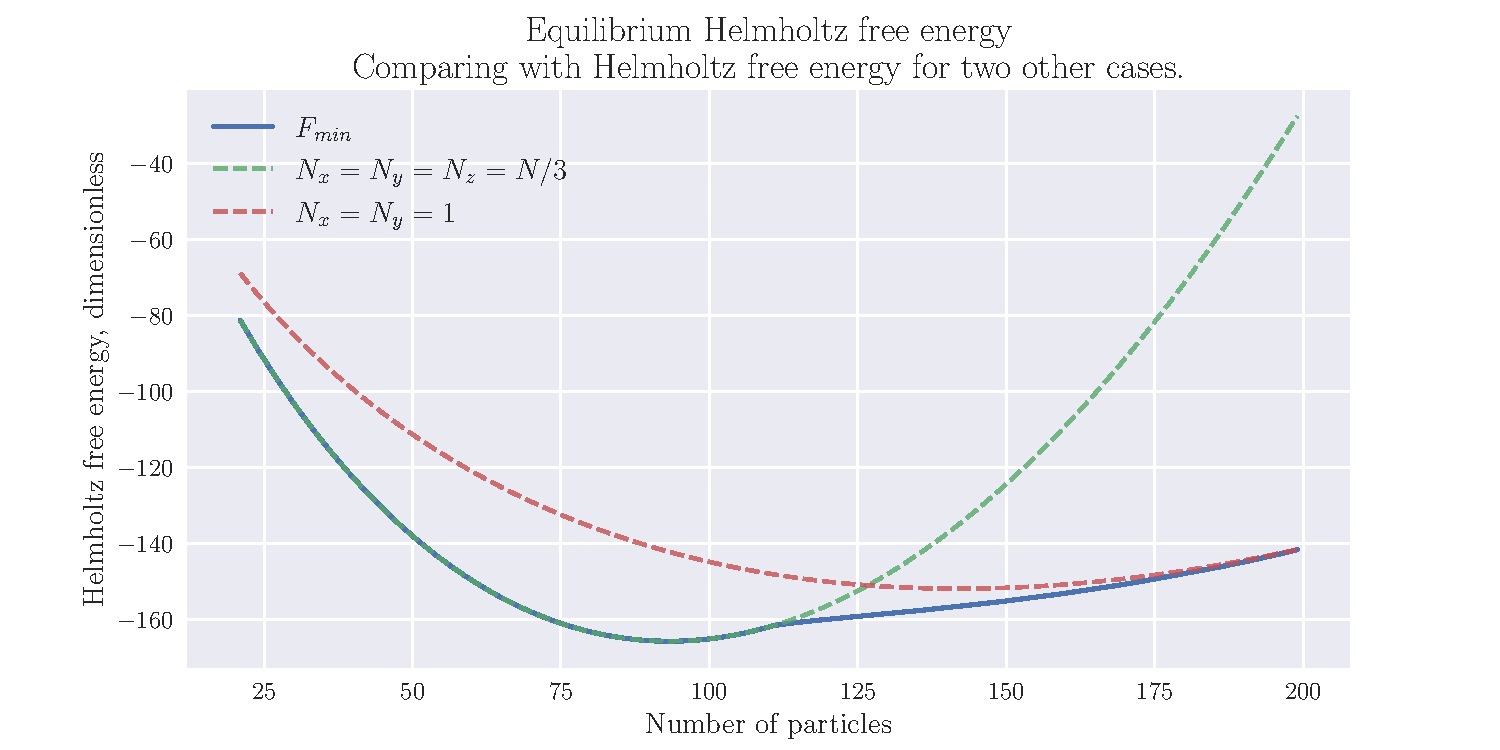
\includegraphics[width=0.8\linewidth]{helmholtz_free_energy.pdf}
	\caption{Helmholtz}
	\label{fig:F}
\end{figure}


PRESSURE 


\begin{figure}[h!]
	\centering
	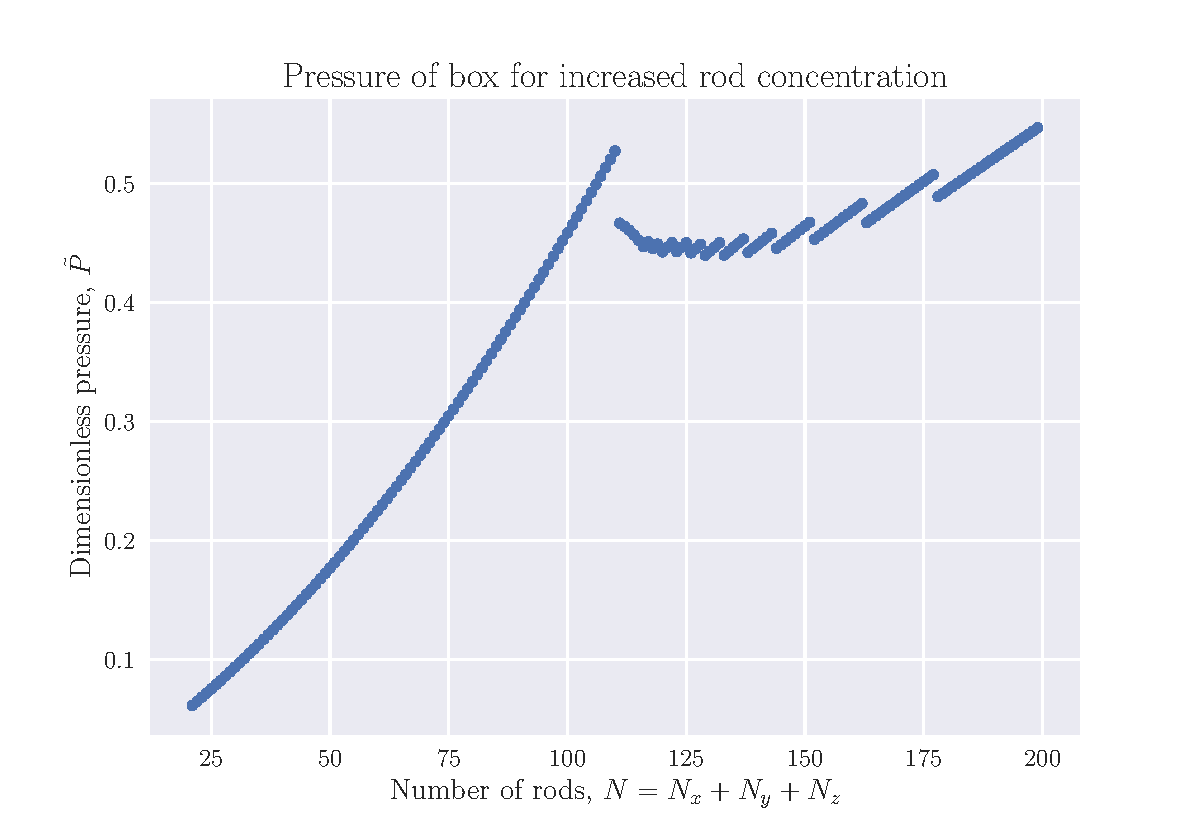
\includegraphics[width=0.8\linewidth]{helmholtz_pressure.pdf}
	\caption{Helmholtz}
	\label{fig:F_P}
\end{figure}


NUMBER DENSITY 



\subsection*{c) - Equilibrium Gibbs free energy}
The Gibbs free energy is given as $G=F+PV$. We find an expression for the pressure, by taking the partial derivative of $F$ with respect to volume, at constant $T$ and $N$
\begin{align*}
	P &= -\tmdv{F}{V}{T}{N} = -\tmdv{\V}{V}{T}{N}\tmdv{F}{\V}{T}{N}=-\frac{1}{lb^2}\tmdv{F}{\V}{T}{N}
\end{align*}
We now define the dimensionless pressure, $\P\equiv Plb^2/T$, and can then differentiate equation \eqref{eq:F_dimless} with respect to $\V$.
\begin{align*}
	\P &= -\bracket{-\frac{\nx}{\V} -\frac{\ny}{\V} -\frac{\nz}{\V} - \gamma \frac{\nx\ny+\ny\nz+\nz\nx}{\V^2}} \\ 
	& = \frac{N}{\V} + \gamma \frac{\nx\ny+\ny\nz+\nz\nx}{\V^2} 
\end{align*}
We can now find the dimesnionless Gibbs free energy, $G/T$
\begin{align*}
	\frac{G}{T} &= \frac{F}{T} + \frac{PV}{T} = \frac{F}{T} + \P\V \\
	&= N_x \ln\closed{\frac{N_x}{\tilde{V}}} + N_y \ln\closed{\frac{N_y}{\tilde{V}}} + N_z \ln\closed{\frac{N_z}{\tilde{V}}} + 2\gamma \frac{\nx\ny+\ny\nz+\nz\nx}{\tilde{V}} + N 
\end{align*}


\section*{\large Task 4}

\begin{align} \label{eq:task4_energy}
	E=J(\np-N_-)
\end{align}

\subsection*{a)}
The system we're considering is analogous to a toin coss, and we find the number of different micrstates from the binomial coefficient, where the constrain $\np+N_-=N$ can be used to eliminate $N_-$
\begin{align*}
	\Omega(N,\np) = \frac{N!}{\np!N_-!}=\frac{N!}{\np!(N-\np)!}
\end{align*}


\subsection*{b)}
To find the entropy as a function for $T$ and $N$ where we assume large $N$, we start by taking the logarithm of $\Omega(N,\np)$ and use Stirling's approximation on the different terms. 
\begin{align*}
	\ln\Omega(N,\np) &= \ln(N!) - \ln(\np!)-\ln(N-\np)! \\ 
	&\approx N\ln N - \np \ln\np - (N-\np)\ln(N-\np) - N + \np + (N-\np) \\
	&=N\ln N - \np \ln\np - (N-\np)\ln(N-\np)
\end{align*}
We want to eliminate $\np$ from the expression in favor of temperature. To do this, we will take the partial derivative of $S$ with respect to $E$
\begin{align*}
	\frac{1}{T}=\tmdv{S}{E}{V}{N}=\tmdv{\np}{E}{V}{N}\tmdv{S}{\np}{V}{N}
\end{align*}
Rewriting equation \eqref{eq:task4_energy} in terms of $\np$ and $N$ yields an expression for the derivative of $\np$ with respect to $E$
\begin{align*}
	E = J(2\np-N) \implies& \np = \frac{1}{2}\closed{\frac{E}{J}+N} \\ 
	\tmdv{\np}{E}{V}{N} =&\;\; \frac{1}{2J}
\end{align*}
Using the definition of entropy, $S = \kb \ln\Omega(N,\np)$, we differentiate that with respect to $\np$, where we use the approximated expression for $\ln\Omega(N,\np)$

\begin{align*}
	\tmdv{S}{\np}{V}{N} &= \kb \pdv{\np}\bracket{N\ln N - \np\ln\np - (N-\np)\ln(N-\np)} \\ 
	&= \kb \bracket{-\ln\np - 1 + \ln(N-\np) + 1} \\ 
	&= \kb\ln\closed{\frac{N-\np}{\np}}
\end{align*}
Putting the pieces back together, we get 
\begin{align*}
	\frac{1}{T} &= \frac{1}{2J} \kb \ln\closed{\frac{N-\np}{\np}} \\ 
	\ln\closed{\frac{N-\np}{\np}} &=\frac{2J}{\kb T} \\ 
	\implies \np = \frac{N}{1+e^{2J/\kb T}}
\end{align*}
For simplicity, we now define $x\equiv \frac{2J}{\kb T}$. Before we start inserting our expression for $\np$ to obtain the entropy function we find expressions for $\ln\np$, $N-\np$ and $\ln(N-\np)$ in terms of $N$ and $x$. 
\begin{align*}
	\ln\np&=\ln\closed{\frac{N}{1+e^x}} = \ln N - \ln(1+e^x) \\ 
	N - \np &= N\closed{1 - \frac{1}{1+e^x}}=N\closed{\frac{e^x}{1+e^x}}=\frac{N}{1+e^{-x}} \\
	\ln(N-\np) &= \ln\closed{\frac{N}{1+e^{-x}}} = \ln N - \ln(1+e^{-x})
\end{align*}  

Inserting these values for $\ln\Omega(N,\np)$ yields 
\begin{align*}
	S=\kb \ln\Omega(N,\np) &= \kb \bracket{N\ln N - \frac{N}{1+e^x}\closed{\ln N - \ln(1+e^x)} - \frac{N}{1+e^{-x}} \closed{\ln N - \ln(1+e^{-x})}} \\ 
	&=\kb \bracket{N\ln N \closed{1 - \frac{1}{1+e^x} - \frac{1}{1+e^{-x}}} + N\closed{\frac{\ln(1+e^x)}{1+e^x} + \frac{\ln(1+e^{-x})}{1+e^{-x}}}} \\ 
	&= N\kb \bracket{\frac{\ln(1+e^x)}{1+e^x} + \frac{\ln(1+e^{-x})}{1+e^{-x}}}
\end{align*}
To proceed, we simplify further by considering the logarithm in the last term 
\begin{align*}
	\ln(1+e^{-x}) &= \ln(e^{-x}(1+e^x)) = -x + \ln(1+e^x) \\ 
	\implies \frac{1}{1+e^{-x}}\ln(1+e^{-x}) &= \frac{\ln(1+e^x)}{1+e^{-x}} - \frac{x}{1+e^{-x}}
\end{align*}
Having two common factors of $\ln(1+e^x)$, the entropy expression simplifies even further 

\begin{align*}
	S &= N\kb \bracket{\closed{\frac{1}{1+e^x} + \frac{1}{1+e^{-x}}}\ln(1+e^x) - \frac{x}{1+e^{-x}}} \\ 
	&= N\kb \bracket{\ln(1+e^x) - \frac{x}{1+e^{-x}}}
\end{align*}

Inserting the expression for $x$ yields the final entropy expression as a function of $T$ and $N$
\begin{align}
	S(T,N) &= N\kb \bracket{\ln\closed{1+e^{2J/\kb T}} - \frac{2J/\kb T}{1+e^{-2J/\kb T}}}
\end{align}

\subsection*{c)}
To find the heat capacity, we use the chain rule to ease the computation 
\begin{align*}
	C_V &= T\tmdv{S}{T}{V}{N} = T \tmdv{x}{T}{V}{N}\tmdv{S}{x}{V}{N} = -T\frac{2J}{\kb T^2}\tmdv{S}{x}{V}{N} \\ 
	\tmdv{S}{x}{V}{N} &= N\kb \bracket{\frac{e^x}{1+e^x} - \frac{1}{1+e^{-x}} -x \frac{e^{-x}}{(1+e^{-x})^2} } \\ 
	&= - N\kb x \frac{e^x}{(1+e^x)^2} = -N\kb \frac{2J}{\kb T} \frac{e^{2J/\kb T}}{\closed{1+e^{2J/\kb T}}^2}
\end{align*}
Putting it all together, we finally arrive at 
\begin{align*}
	C_V = \frac{4J^2 N}{\kb} \frac{1}{T^2} \frac{e^{2J/\kb T}}{\closed{1+e^{2J/\kb T}}^2}
\end{align*}
Without any explicit calculation, we rewrite the exponential factor in terms of a hyperbolic function 
\begin{align*}
	\frac{e^x}{(1+e^x)^2} &= \frac{1}{4\cosh^2(\frac{x}{2})} \\
	\implies \frac{e^{2J/\kb T}}{\closed{1+e^{2J/\kb T}}^2} &= \frac{1}{4 \cosh^2\closed{\frac{J}{\kb T}}}
\end{align*}
And our final expression for the heat capacity becomes 
\begin{align}
	C_V = \frac{J^2 N}{\kb} \frac{1}{T^2} \frac{1}{\cosh^2\closed{\frac{J}{\kb T}}}
\end{align}

\end{document}
